\section{Fit results}
\label{sec:FitResults}

Table \ref{tab:FitParams} shows the measured values for the extracted radii and scattering parameters, along with statistical and systematic error bars.
The "Fit Sys" and "Cut Sys" columns list the systematic uncertainties arising from variation in the fit method and in the topological and pair cut values, respectively.
In almost all cases, the cut systematics are an order of magnitude smaller than the fit method systematics.
The "Total Sys" column shows the fit method and cut systematics added in quadrature.
%While the systematic uncertainties are not directly correlated with the statistical uncertainties, 

\begin{table}
\label{FitResultsTable}
\begin{center}
\begin{tabular}{|l|l|l|l|l|l|}
\hline 
Parameter & Value (fm) & $\pm$ Stat & $\pm$ Total Sys & Fit Sys & Cut Sys \\ 
\hline 
Radius $\Lambda\bar{\Lambda}$ 0-10\% & 2.9 & 0.3 & 0.3 & 0.3 & 0.02 \\ 
\hline 
Radius $\Lambda\bar{\Lambda}$ 10-30\%  & 2.3 & 0.2 & 0.2 & 0.2 & 0.02 \\ 
\hline 
Radius $\Lambda\bar{\Lambda}$ 30-50\%  & 1.8 & 0.2 & 0.2 & 0.2 & 0.01 \\ 
\hline 
Radius $\Lambda\Lambda$ 0-10\% & 5.4 & 0.6 & 0.2 & 0.2 & 0.1 \\ 
\hline 
Radius $\Lambda\Lambda$ 10-30\% & 4.2 & 0.5 & 0.2 & 0.2 & 0.04 \\ 
\hline 
$\Re f_0$ $\Lambda\bar{\Lambda}$ & -0.5 & 0.1 & 0.1 & 0.1 & 0.01 \\ 
\hline 
$\Im f_0$ $\Lambda\bar{\Lambda}$ & 0.14 & 0.09 & 0.02 & 0.02 & 0.006 \\ 
\hline 
$\Re f_0$ $\Lambda\Lambda$ & -0.6 & 0.3 & 0.05 & 0.04 & 0.02 \\ 
\hline 
$d_0$ $\Lambda\bar{\Lambda}$ & 1.7 & 0.2 & 0.2 & 0.2 & 0.01 \\ 
\hline 
$d_0$ $\Lambda\Lambda$ & 5.3 & 2.7 & 0.3 & 0.2 & 0.2 \\ 
\hline 
\end{tabular} 
\end{center}
\caption[Fit results]{Measured fit parameters with statistical and systematic errors.
All values are measured in fm.
The Fit Sys and Cut Sys columns show the systematic uncertainties arising from variations in the fit method and the topological and pair cut parameters, respectively.
The Total Sys column comes from the fit and cut systematic errors added in quadrature. }
\label{tab:FitParams}
\end{table}






%\subsection{Discussion of results}
%\label{sec:ResultsDiscussion}



\subsection{$\Re f_0$}
\label{sec:Ref0Result}


Figure \ref{fig:Ref0} shows the measured $\Re f_0$ for $\Lambda\Lambda$ and $\Lambda\bar{\Lambda}$. A number of other measurements are included for comparison. From the left: $\Lambda\bar{\Lambda}$ and $\Lambda\Lambda \oplus \bar{\Lambda}\bar{\Lambda}$ scattering lengths from this analysis, $\Lambda\Lambda \oplus \bar{\Lambda}\bar{\Lambda}$ from Au--Au $\sqrt{s_{\mathrm{NN}}} = 200\ \mathrm{GeV}/c$ measured at STAR \cite{Adamczyk:2014vca}, $\Lambda\Lambda$ result from a 4-body cluster model of hypernuclear interactions \cite{Hiyama:2002yj} applied to a measurement of $\ce{^{6}_{\Lambda\Lambda}\mathrm{He}}$ \cite{Takahashi:2001nm}, $\Lambda\Lambda$ result from the Nijmegen D soft-core interaction model \cite{Filikhin:2002wm} (also applied to \cite{Hiyama:2002yj}), $\mathrm{p}\bar{\Lambda}$ extracted from a residual correlation analysis \cite{Kisiel:2014mma} of STAR data, $\mathrm{p}\Lambda$ singlet and triplet scattering lengths \cite{Wang:1999bf}, np singlet and triplet scattering lengths \cite{LANDAU1977502}, and the nn scattering length \cite{vonWitsch:1979uni}.

\begin{figure}[hbt]
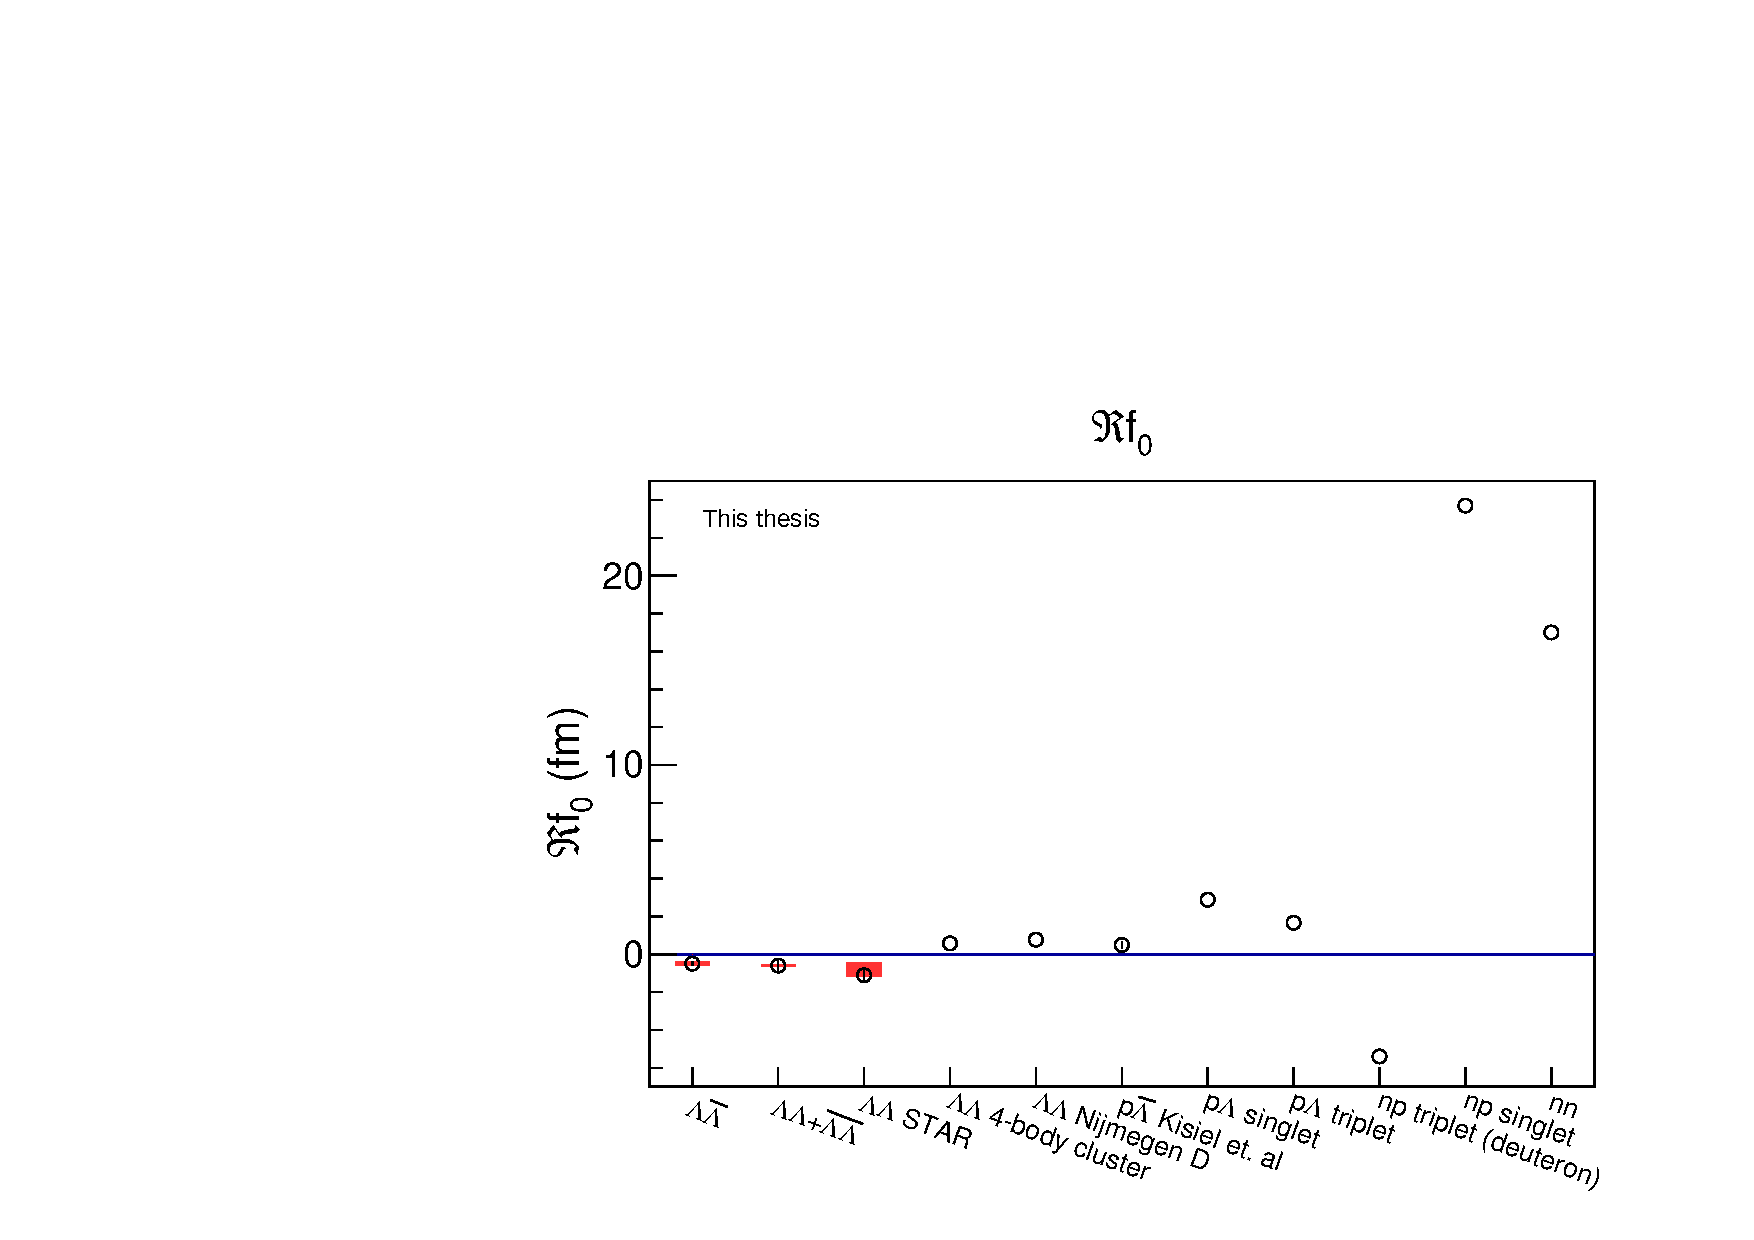
\includegraphics[width=36pc]{Figures/FitResults/2016-10-12-Ref0.pdf}
\caption[Measurements of $\Re f_0$ for various particle pairs]{Several measurements of the real part of the $\Lambda\Lambda$ and $\Lambda\bar{\Lambda}$ scattering lengths. p$\Lambda$, p$\bar{\Lambda}$, np, and nn are included for comparison. The np spin-triplet state --- the deuteron --- is a weakly bound state. The $\Lambda\Lambda$ scattering length is an order of magnitude smaller than the np scattering length, which is evidence that there is no $\Lambda\Lambda$ dibaryon bound state.}
\label{fig:Ref0}
\end{figure}

The np triplet spin state is a known bound state --- the ground state of the deuteron.
Our measurement $\Lambda\Lambda$ scattering length ($\sim-0.6$ fm) is about an order of magnitude smaller than the deuteron scattering length.
Since the deuteron is only weakly bound, the significantly smaller scattering length of $\Lambda\Lambda$ suggests that it does not have a dibaryon bound state.

% Zoomed in picture of the scattering lengths
\begin{figure}[hbt]
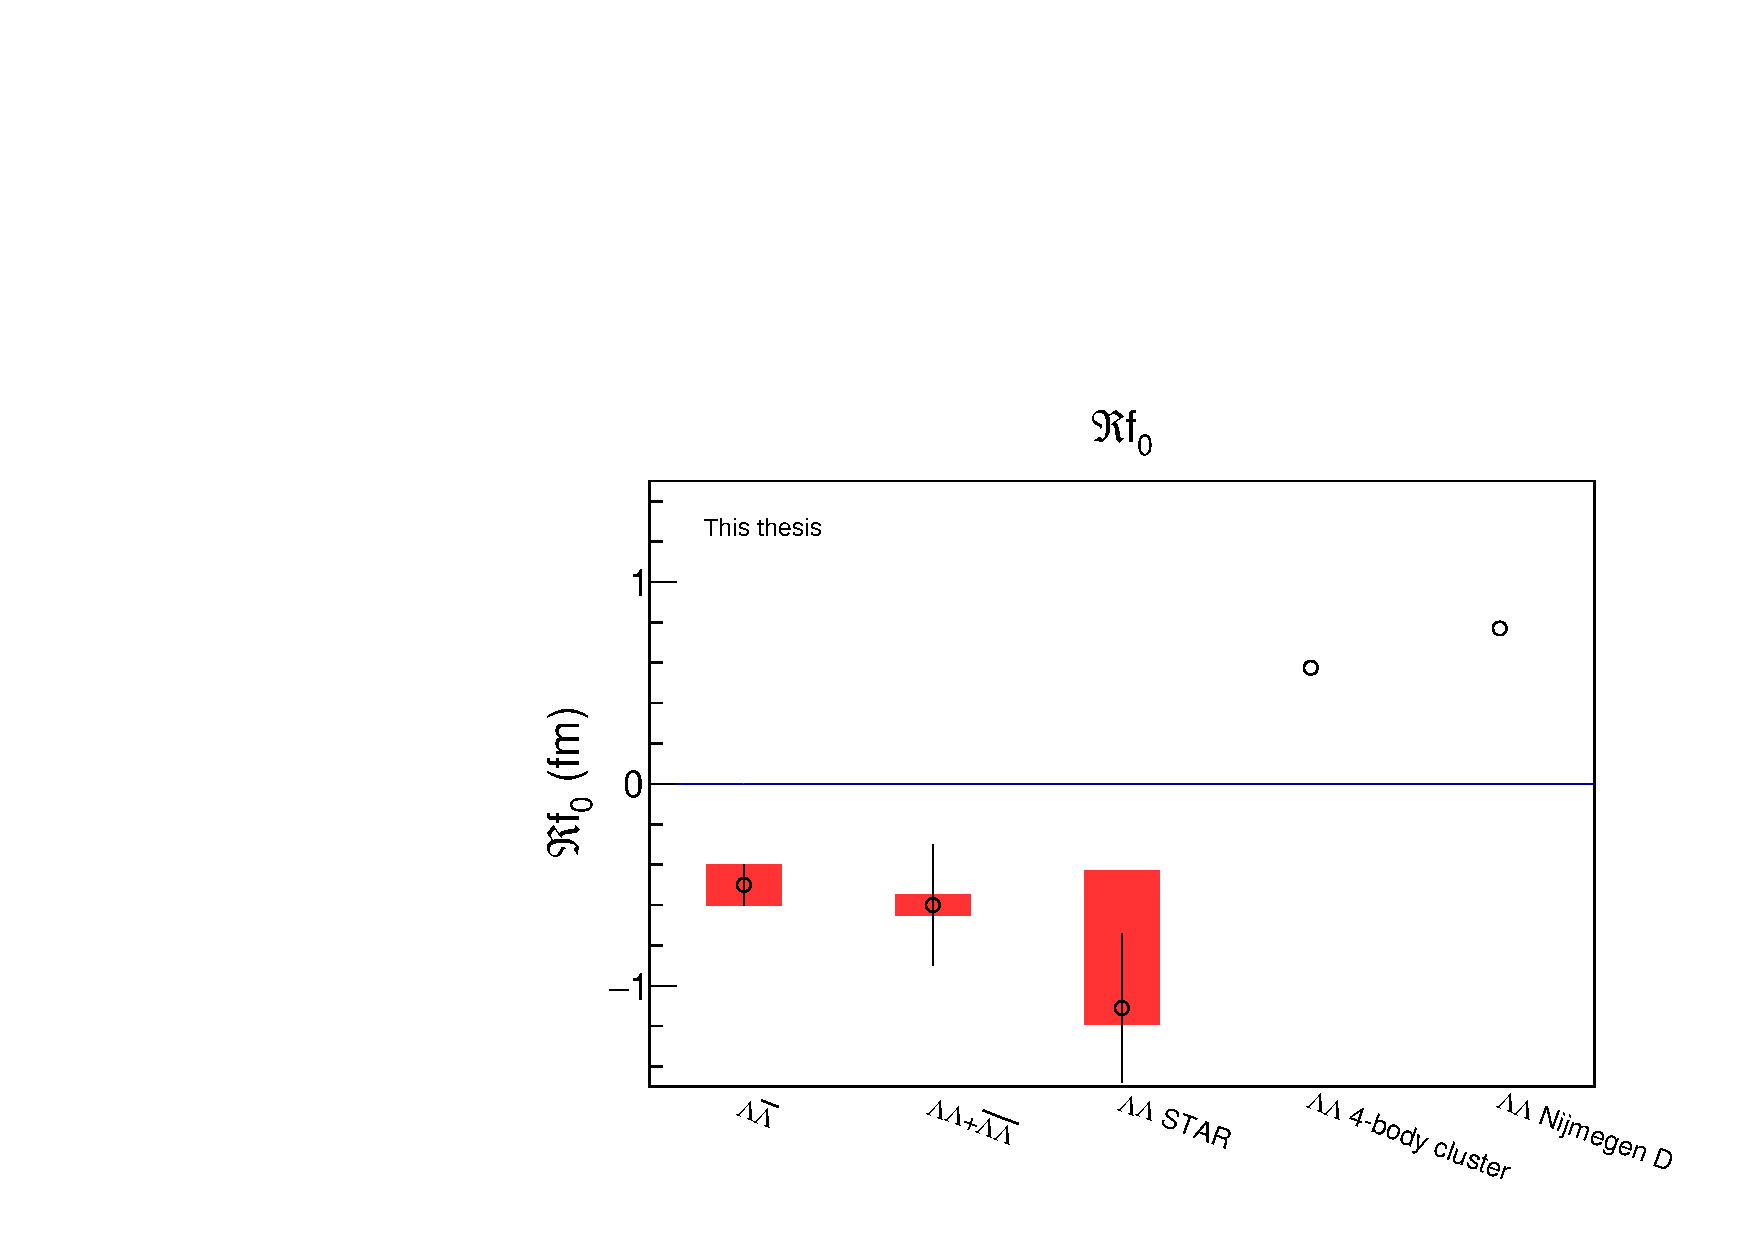
\includegraphics[width=36pc]{Figures/FitResults/2016-10-12-Ref0Zoom.pdf}
\caption[Measurements of $\Re f_0$ for various particle pairs (zoomed)]{Several measurements of the real part of the $\Lambda\Lambda$ and $\Lambda\bar{\Lambda}$ scattering lengths. The STAR measurement \cite{Adamczyk:2014vca} of the $\Lambda\Lambda$ scattering length agrees with our measurement within their systematic uncertainty. Our measurement is similar in magnitude but opposite the sign of $\Lambda\Lambda$ scattering lengths calculated from hypernuclear structure models \cite{ Hiyama:2002yj, Filikhin:2002wm} applied to a measured $\ce{^{6}_{\Lambda\Lambda}\mathrm{He}}$ nucleus \cite{Takahashi:2001nm}.}
\label{fig:Ref0Zoom}
\end{figure}

Figure \ref{fig:Ref0Zoom} shows $\Re f_0$ again, but here it is zoomed in to better highlight the details of the various $\Lambda\Lambda$ measurements.
There are several features to note here.
First, our measured real scattering length for $\Lambda\Lambda\oplus\bar{\Lambda}\bar{\Lambda}$ is consistent with that for $\Lambda\bar{\Lambda}$.
This suggests that their behavior under elastic scattering is the same; only the annihilation of the $\Lambda\bar{\Lambda}$ pair (accounted for by the imaginary part of the scattering length) sets them apart.

Second, we can see that the STAR measurement of $\Lambda\Lambda$ agrees with our measurement within their systematic uncertainties.
That said, neither our measurement nor STAR's agrees with the results from the hypernuclear interaction models.
While they are of a similar magnitude, the hypernuclear scattering results have a positive sign, suggesting an attractive interaction rather than repulsive.

\subsection{$\Im f_0$}
\label{Imf0Result}

The few measured baryon-antibaryon scattering lengths have imaginary components on the order of 1 fm.
The imaginary part of the $\mathrm{p\bar{p}}$ scattering length has been measured to be $\Im f_{0,\mathrm{p\bar{p}}} = 0.95 \pm 0.12$ fm, and the value for $\mathrm{p\bar{n}}$ is $\Im f_{0,\mathrm{p\bar{n}}} = 0.83 \pm 0.07$ fm \cite{Mutchler:1988av}. 
Analysis of the STAR $\mathrm{p\bar{\Lambda} \oplus \bar{p}\Lambda}$ correlation functions in 200 GeV Au--Au \cite{Adams:2005ws} collisions with (without) accounting for residual correlations yields $\Im f_{0,\mathrm{p\bar{\Lambda}}} = 0.82 \pm 0.28$ fm ($\Im f_{0,\mathrm{p\bar{\Lambda}}} = 1.00 \pm 0.21$ fm) \cite{Kisiel:2014mma}.
It has been hypothesized that baryon-antibaryon pairs in general may have similar annihilation cross sections at comparable relative momentum \cite{Kisiel:2014mma}.
Indeed, as many $\mathrm{B\bar{B}}$ interactions are unknown, the UrQMD model treats all annihilation cross-sections as being the same as the $\mathrm{p\bar{p}}$ annihilation cross-section at the same $\sqrt{s}$ \cite{Bleicher:1999xi}.
In contrast with these various measurements and models, our measured scattering length is $\Im f_{0,\Lambda\bar{\Lambda}} = 0.14 \pm 0.09\ (\mathrm{stat}) \pm 0.02\ (\mathrm{sys})$ fm, about a factor of 6 smaller than the other values.

\subsection{$d_0$}
% d0

$d_0$ enters into the wave function as a correction to the scattering amplitude, and in general it has a less profound effect on the correlation function than the scattering length.
There are a few different treatments of $d_0$ across the field of research.
When the value is known, such as for pp femtoscopy \cite{Adam:2015vja}, it implemented as a fixed value in the fits.
In other cases, it has been set to zero to reduce the number of free fit parameters and avoid over-fitting \cite{Kisiel:2014mma, Shapoval:2014yha, Adams:2005ws}.
In this analysis as well as the the STAR analyses of $\mathrm{\bar{p}\bar{p}}$ and $\Lambda\Lambda$ correlations \cite{Adamczyk:2015hza, Adamczyk:2014vca}, $d_0$ is left as a free parameter with the intention of letting nature tell whatever story it wants to tell.

The moral of that story seems to be that $d_0$ is not very well constrained. 
We obtained $d_{0,\Lambda\Lambda} =  5.3\ \mathrm{fm} \pm 2.7\ \mathrm{(stat)} \pm 0.3\ \mathrm{(sys)}$ --- about 50\% uncertainty.
For $\Lambda\bar{\Lambda}$, we faired better with 17\% uncertainty: $d_{0,\Lambda\bar{\Lambda}} =  1.7\ \mathrm{fm} \pm 0.2\ \mathrm{(stat)} \pm 0.2\ \mathrm{(sys)}$.
STAR measured a larger effective range $d_{0,\Lambda\Lambda} =  8.52\ \mathrm{fm} \pm 2.56\ \mathrm{(stat)}^{+2.09}_{-0.74}\ \mathrm{(sys)}$ --- about 30--40\% uncertainty.
And for their recent measurement of the $\mathrm{\bar{p}\bar{p}}$ interaction, they found $d_{0,\bar{\mathrm{p}}\bar{\mathrm{p}}} = 2.14\ \mathrm{fm} \pm 0.27\ \mathrm{(stat)} \pm 1.34\ \mathrm{(sys)}$ --- about 60\% uncertainty. 

While the uncertainties are all fairly large, the measured values are at least in the same ballpark as the effective range values measured for low-energy nucleon-nucleon scattering, all of which lie in the 2.5 to 3 fm range \cite{Noyes:1973zd}.
This suggests that it isn't hopeless to try to extract $d_0$ from femtoscopic analyses, but those analyses will need more statistics than are available for $\Lambda\Lambda$ at this time.

\subsection{Radii}

Figure \ref{fig:RvsMt} shows the extracted 1D radii $R_{\mathrm{inv}}$ for $\Lambda\Lambda\oplus\bar{\Lambda}\bar{\Lambda}$ and $\Lambda\bar{\Lambda}$ as a function of centrality and the average transverse mass $m_{\mathrm{T}}$ of the measured pairs.
Also included are the radii for $\pi^\pm\pi^\pm$, $\mathrm{K^\pm}\mathrm{K^\pm}$, $\mathrm{K^0_S}\mathrm{K^0_S}$, pp, $\bar{\mathrm{p}}\bar{\mathrm{p}}$ \cite{Adam:2015vja}, and p$\Lambda\oplus\bar{\mathrm{p}}\bar{\Lambda}$ (unpublished, \cite{Beck:2015msi}).
With $R_{\Lambda\bar{\Lambda},0-10\%} = 2.9\pm 0.3 \pm 0.3$ fm, $R_{\Lambda\bar{\Lambda},10-30\%} = 2.3\pm 0.2 \pm 0.2$ fm, and $R_{\Lambda\bar{\Lambda},30-50\%} = 1.8\pm 0.2 \pm 0.2$ fm, the $\Lambda\bar{\Lambda}$ points seem to follow the $m_\mathrm{T}$ scaling of the pions, kaons, and protons.
The $\Lambda\Lambda$ and p$\Lambda$ radii are quite large however, and while they are consistent with each other, they do not follow the $m_\mathrm{T}$ scaling trend.


%We do not yet have a good explanation of this phenomena.
%Nor can we explain why the $\Lambda\Lambda\oplus\bar{\Lambda}\bar{\Lambda}$ and $\Lambda\bar{\Lambda}$ radii are so different.


\begin{figure}[hbt]
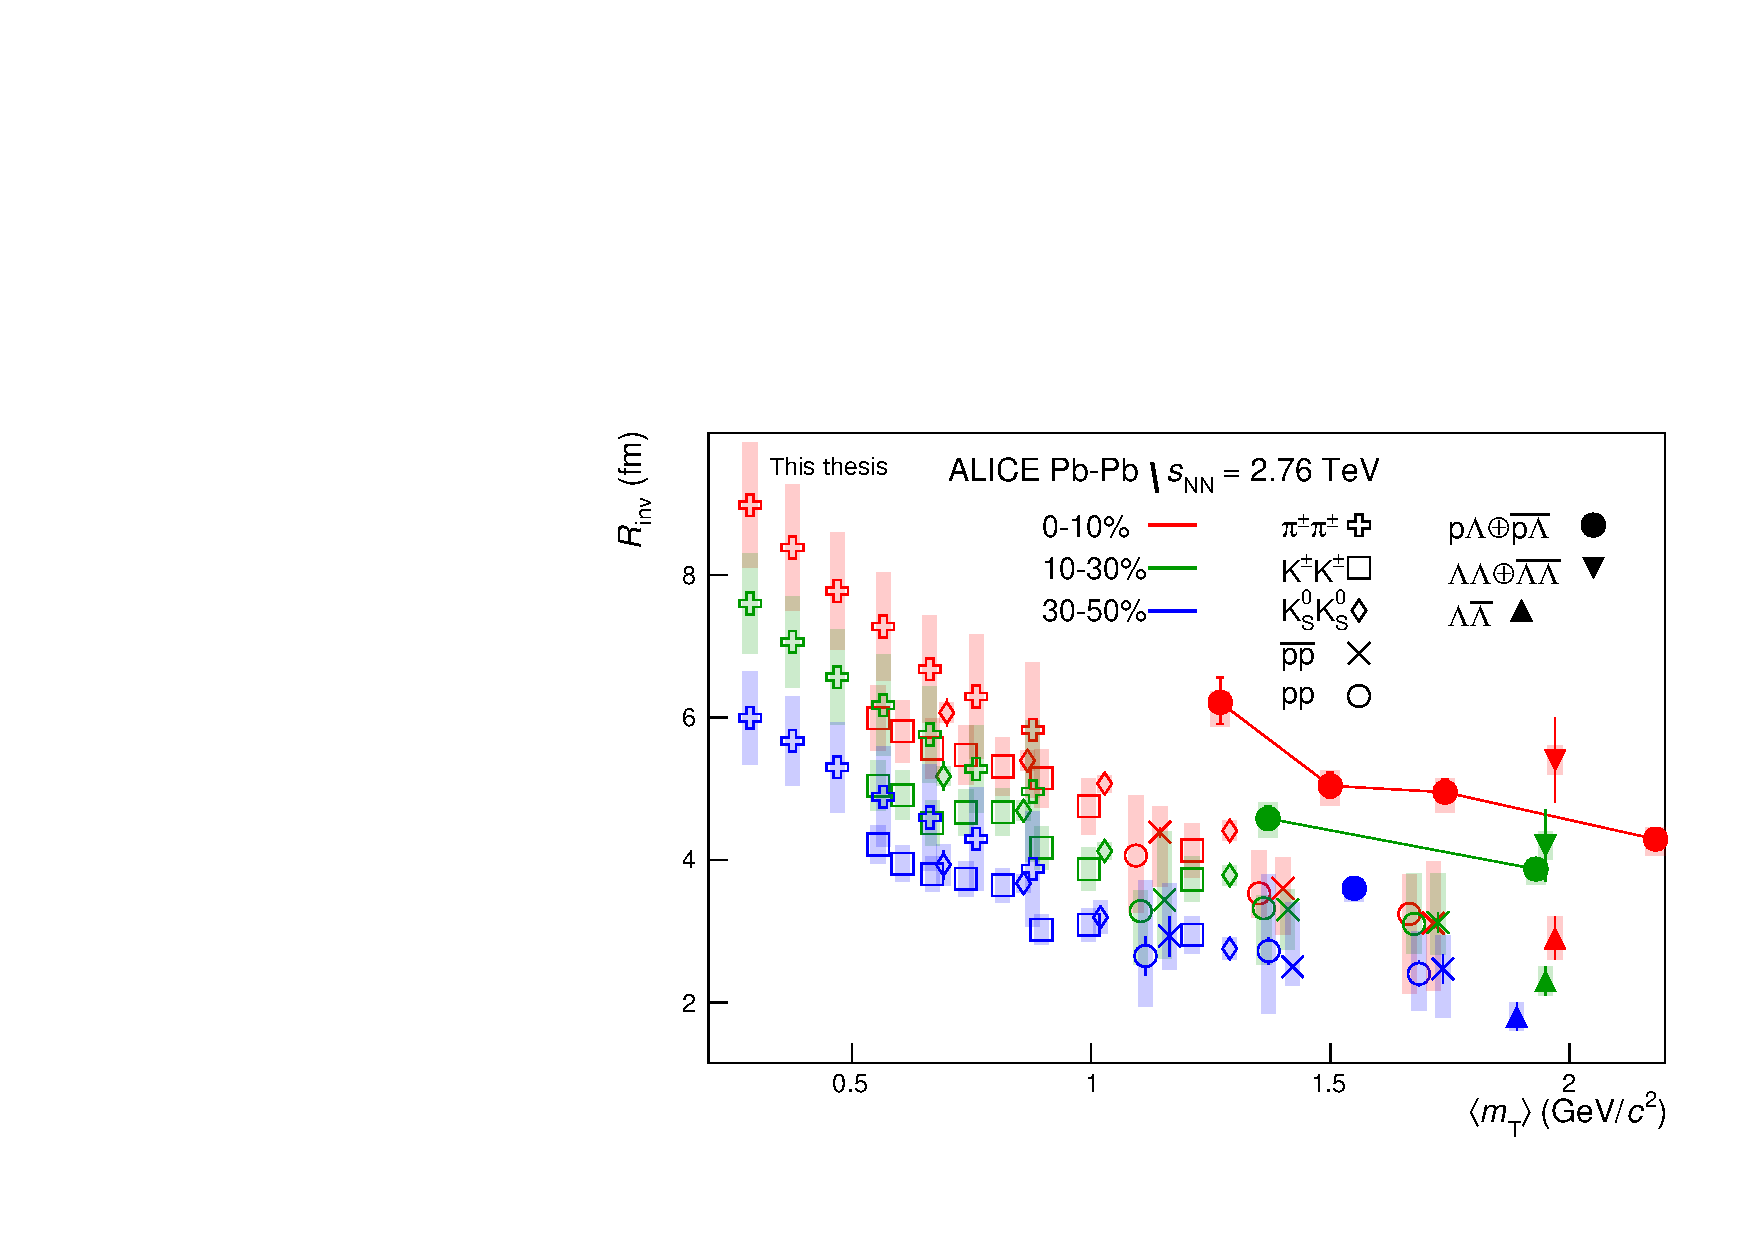
\includegraphics[width=36pc]{Figures/FitResults/2016-09-29-mTscaling.pdf}
\caption[$R_{\mathrm{inv}}$ vs $m_{\mathrm{T}}$]{1D radius $R_\mathrm{inv}$ vs transverse mass $m_\mathrm{T}$ for many different pairs measured by ALICE in $\sqrt{s_\mathrm{NN}} = 2.76$ TeV Pb-Pb collisions \cite{Adam:2015vja}.
The $\Lambda\bar{\Lambda}$ radii appear to follow the trend of $m_\mathrm{T}$-scaling \cite{Csorgo:1995bi,Lisa:2005dd}, but not $\Lambda\Lambda\oplus\bar{\Lambda}\bar{\Lambda}$ or $\mathrm{p}\Lambda\oplus\bar{\mathrm{p}}\bar{\Lambda}$ (unpublished, \cite{Beck:2015msi}).
}
\label{fig:RvsMt}
\end{figure}

There are two peculiar details in these results that need explanation.
What kind of effect would introduce an asymmetry between the particle-particle radius and the particle-antiparticle radius? 
Furthermore, why do the particle-particle radii deviate so much from the loose $m_\mathrm{T}$ trend observed for the pions, kaons, and protons?
An ideal explanation would answer both of these questions with a single effect (e.g.\ perhaps there is some unaccounted for detector effect modifying the $\Lambda\Lambda\oplus\bar{\Lambda}\bar{\Lambda}$ correlation function in such a way as to make the radius appear larger).
If the measured results are correct, we would like to identify the underlying physics.
If the measured results are incorrect, we want to determine where the problem lies in the experimental method or analysis process.
In what follows, we will offer several hypotheses for why these results are seen, but first, let us discuss why the difference in radii is unusual.

If one considers the two-particle emission functions to be simple convolutions of the single-particle $\Lambda$ and $\bar{\Lambda}$ emission functions, and one assumes that there is no asymmetry between those single-particle emission functions at the $\sqrt{s}$ and $\mu_b$ of the LHC, then in the absence of other confounding effects one would assume that $\Lambda\Lambda$, $\bar{\Lambda}\bar{\Lambda}$, and $\Lambda\bar{\Lambda}$ would all have the two-particle emission functions and same radii.
While the $\Lambda\Lambda$ and $\bar{\Lambda}\bar{\Lambda}$ correlation functions and radii are consistent with each other, we see that the $\Lambda\Lambda\oplus\bar{\Lambda}\bar{\Lambda}$ radii are larger than the comparable centrality $\Lambda\bar{\Lambda}$ radii by almost a factor of two.

It is possible that the anomalous differences between the $\Lambda\Lambda\oplus\bar{\Lambda}\bar{\Lambda}$ and $\Lambda\bar{\Lambda}$ radii may an error introduced by over- or under-corrected detector effects such as splitting and merging.
If this is to blame, it would probably afflict the $\Lambda\Lambda\oplus\bar{\Lambda}\bar{\Lambda}$ correlation functions.
The $\Lambda\bar{\Lambda}$ correlation function is fairly robust against such effects. 
The correlation function is very wide, while splitting/merging affects the low-$k^*$ range.
In addition, for detector effects to occur with same-sign particles in $\Lambda\bar{\Lambda}$, a proton would have to be identified as a pion or vice versa.

So given the cuts implemented in Section \ref{sec:PairWiseCuts}, why might there still be an issue?
In short, it is possible that real correlated physics effects might show up in our average separation correlation functions.
In that case, when we set our pair cuts to remove merging, we may have accidentally cut out physics effects as well.

%Well, first let's elaborate on the discussion of pair cuts from .
There is some correlation between the measured positions of charged tracks and the momenta of those tracks and their parents.
Through that correlation, the detector effects of splitting and merging can show up as false signals in relative momentum correlation functions.
It may be the case that true physics correlations can show up as false signals in average separation correlation functions, the purpose of which is to detect and remove splitting and merging.
If true physics effects bleed into the average separation plots, it may lead us to impose strict cuts which unintentionally remove those physics effects from the femtoscopic correlation functions.
Such a cut may lead to spurious fit results, such as the anomalously large $\Lambda\bar{\Lambda}\oplus\bar{\Lambda}\bar{\Lambda}$ radii.
Future analyses may find merit in investigating alternative criteria to cut upon.
For example, one might require the decay lengths of the V0s to differ by several centimeters.
This would bias the daughter tracks to a larger separation, thus limiting splitting and merging effects, without introducing any relative momentum bias.
Then it seems the risk of unintentionally cutting out true physics effects would be small, as it is unlikely that there is any correlation between the relative momentum of particles and their relative decay positions.

Of course, it is also possible that the radius results presented here are correct, that there truly is a physical difference between the emission functions of $\Lambda\Lambda$/$\bar{\Lambda}\bar{\Lambda}$ and $\Lambda\bar{\Lambda}$.
One way this might occur would be if the $\Lambda\bar{\Lambda}$ two-particle emission function contains a sizable number of pairs coming from pair creation.

For example, near-threshold pair creation of $\Lambda\bar{\Lambda}$ particles could cause low-$k^*$ pairs to be emitted with only a small spatial separation.
If there are a sizable number of these pairs, the two-particle emission function would have an additional component with a small radius, similar to the core-halo effect in pion femtoscopy (in addition to the usual Gaussian signal measured in pion correlation functions, there is also a very narrow enhancement in the lowest few $k^*$ bins arising from a very large emission region, the pions that come from the decays of long-lived resonances).
In the $\Lambda\bar{\Lambda}$ case, the two-particle emission function would have a component with a small radius from the pair-created particles, as well the expected "normal"-sized radius component arising from the convolution of the two single-particle emission functions.

The fit function we employ only has one radius parameter, not two, so the single radius radius may be something of an average of the size of these two regions.
Because of that, the extracted $\Lambda\bar{\Lambda}$ radius would be smaller than the radius of either of the $\Lambda$ or $\bar{\Lambda}$ single-particle emission functions, and thus smaller than the $\Lambda\Lambda\oplus\bar{\Lambda}\bar{\Lambda}$ radius.
While this would account for a discrepancy between the particle-particle and particle-antiparticle radii, it seems like it would result in the $\Lambda\bar{\Lambda}$ radii looking too small, rather than the $\Lambda\Lambda\oplus\bar{\Lambda}\bar{\Lambda}$ radii looking too big.
When STAR was trying to account for the difference between the p$\Lambda$ and p$\bar{\Lambda}$ radii, they conjectured that pair creation might have something to do it \cite{Adams:2005ws}.
But in their case, the particle-antiparticle radius looked too small, as would be expected from this effect.

These are a couple potential explanations for our curious results.
It seems like the former issue, better treatment of detector effects, would be the best avenue to explore next, since it could account for the large $\Lambda\Lambda\oplus\bar{\Lambda}\bar{\Lambda}$ radii.
The latter issue, pair creation giving rise to complicated emission functions, could possibly be explored by analyzing emission positions of particles in UrQMD.

% Plot with STAR radii

% unclear background treatment. Some experiments have alleviated some of the background effects incorporating event-plane binning into their correlation function construction.